\begin{frame}{Summary}
    \textbf{Use} : Analysis of high-dimensional data by automatically extracts sparse and meaningful features from a set of nonnegative data vectors\\
    ~\\
    %\begin{figure}
     %   \centering
      %  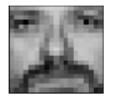
\includegraphics[width=2cm]{face_image.png}
    %\end{figure}
    %Data matrix : $X\in\real^{p\times n}_+$\\
    \begin{enumerate}
        \item What : Definitions as introduction
        \item Why : Applications
        \item How : Formal view and algorithmic difficulties
        \item What next : Connections to other problems %in Mathematics and Computer Science
        \item Conclusion
    \end{enumerate}
\end{frame}

\begin{frame}{What : Definitions and properties}
     Nonnegative matrix factorization (NMF) is a Linear dimensionality reduction (LDR) \\
         ~\\
         % introduced by Paatero and Tapper in 1994 and more developped by Lee and Seung in 1999
         

     \textbf{NMF} : decomposing a given nonnegative data matrix $X$ as $X \approx W H$ where $W \geq 0$ and $H \geq 0$ %component-wise nonnegative
     
          ~\\
          
     \textbf{LDR} : \\
     \begin{itemize}
         \item From a set of data points $x_j \in R^{p}$ for $1 \leq j \leq n$ 
         \item To a set of dimension $r < min(p,n)$
         \item Thanks to $w_k \in R^p$ for $1 \leq k \leq r$
         \item Such that : $\forall j, x_j \approx \sum_{k = 1}^{r} w_{k} h_{j}(k)$, for some weights $h_j\in R^r$
     \end{itemize}
              ~\\
     Equivalent to \textbf{low-rank matrix approximation} : $X \approx W H$\\
     
     \centering
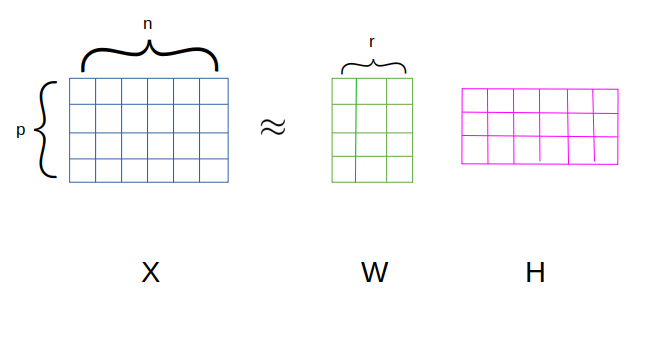
\includegraphics[scale=0.28]{../images/matrices.png}

%     \begin{itemize}
 %    \item $X \in R^{p \times n}$ : $X(:,j) = x_j$ for $1 \leq j \leq n$ %each column of the matrix $X \in R^{p x n}$ is a data point
  %   \item $W \in R^{p \times r}$ : $W(:,k) = w_k$ for $1 \leq k \leq r$ %each column of the matrix $W \in R^{p x r}$ is a basis element
   %  \item $H \in R^{r \times n}$ : $H(:,j) = h_j$ for $1 \leq j \leq n$ %each column of the matrix H gives the coordinates of a data point X(:,j) in the basis W
    % \end{itemize}

\end{frame}
